% !TeX program = pdflatex
% Compile:  tectonic report.tex          (or pdflatex report.tex, twice)
\documentclass[11pt]{article}

\usepackage[margin=1in]{geometry}
\usepackage{microtype, parskip}
\usepackage{amsmath, amssymb, mathtools}
\usepackage{booktabs, siunitx}
\usepackage{caption, subcaption}
\usepackage{xcolor}
\usepackage[hyphens]{url}
\usepackage[hidelinks]{hyperref}
\usepackage{tikz}
\usetikzlibrary{positioning, arrows.meta, calc, shapes.geometric}
\usepackage{graphicx}
\usepackage{listings}

\Urlmuskip=0mu plus 1mu\relax

\lstset{
  basicstyle=\ttfamily\footnotesize,
  breaklines=true,
  showstringspaces=false,
  backgroundcolor=\color{black!4},
  frame=single, framerule=0pt,
  xleftmargin=4pt, xrightmargin=4pt,
}

\title{\bfseries Framewise displacement (FD) vs each\\
electrogastrogram (EGG) channel}
\author{}
\date{}

\begin{document}
\maketitle

\section{Goal}

The main pipeline uses a single dominant electrogastrogram (EGG) channel
(the one with the highest in-band power) selected during preprocessing.
Here we look at all four channels to check two things:

\begin{enumerate}
\item How framewise displacement (FD, Power et al.\ 2012) relates to
each individual EGG channel.
\item Whether the choice of dominant channel affects the FD vs EGG
coupling result.
\end{enumerate}

The implementation lives in \texttt{fwd\_vs\_each\_egg\_channel.py};
outputs are in \path{outputs/}.

\section{Pipeline}

\begin{figure}[h!]
\centering
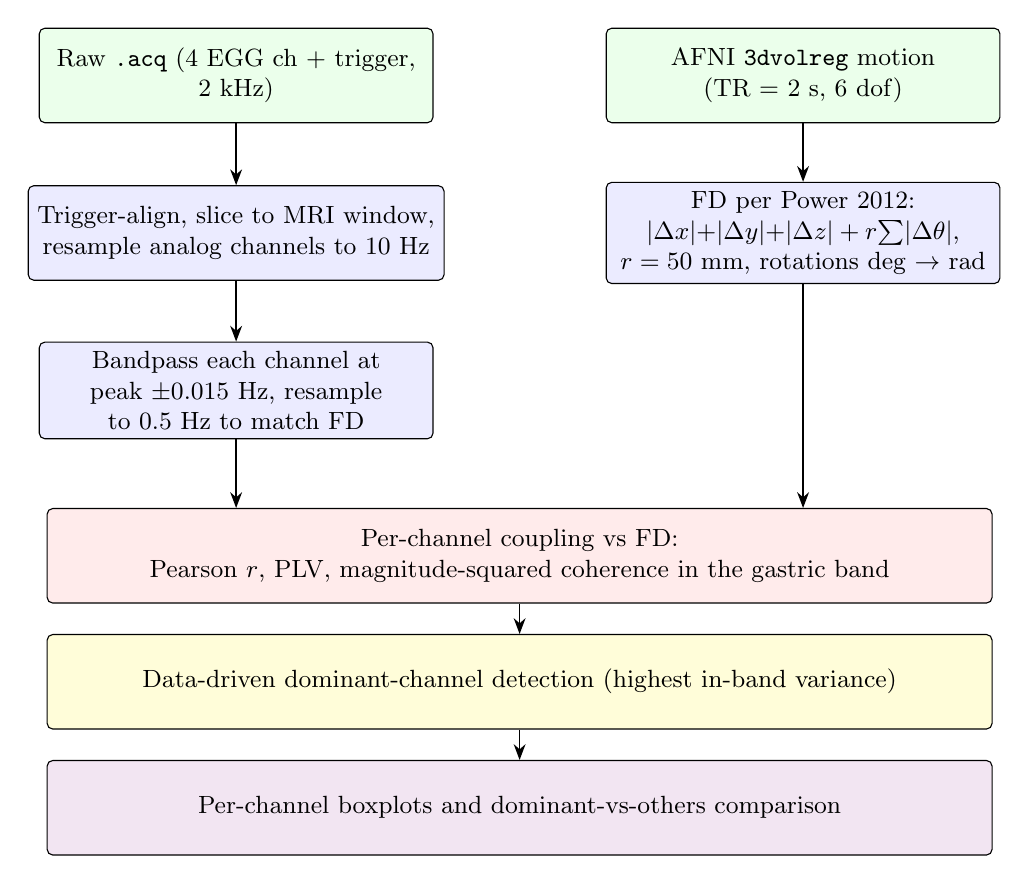
\begin{tikzpicture}[
  x=1cm, y=1cm,
  block/.style={rectangle, draw, fill=blue!8, rounded corners=2pt,
                minimum height=12mm, minimum width=50mm, align=center,
                font=\small},
  data/.style={rectangle, draw, fill=green!8, rounded corners=2pt,
               minimum height=12mm, minimum width=50mm, align=center,
               font=\small},
  wide/.style={rectangle, draw, rounded corners=2pt,
               minimum height=12mm, minimum width=120mm, align=center,
               font=\small},
  arrow/.style={-Stealth, semithick},
]

\node[data] at (-3.6, 0)   (acq)    {Raw \texttt{.acq} (4 EGG ch + trigger,\\2 kHz)};
\node[data] at ( 3.6, 0)   (motion) {AFNI \texttt{3dvolreg} motion\\(TR = 2 s, 6 dof)};

\node[block] at (-3.6, -2.0) (slice)  {Trigger-align, slice to MRI window,\\resample analog channels to 10 Hz};
\node[block] at ( 3.6, -2.0) (fd)     {FD per Power 2012:\\$|\Delta x|{+}|\Delta y|{+}|\Delta z| + r\!\sum\!|\Delta\theta|$,\\$r=50$~mm, rotations deg $\to$ rad};

\node[block] at (-3.6, -4.0) (bp)     {Bandpass each channel at\\peak $\pm 0.015$~Hz, resample\\to 0.5 Hz to match FD};

\node[wide, fill=red!8]     at (0, -6.1) (couple) {Per-channel coupling vs FD:\\
  Pearson $r$, PLV, magnitude-squared coherence in the gastric band};
\node[wide, fill=yellow!15] at (0, -7.7) (dom)    {Data-driven dominant-channel detection (highest in-band variance)};
\node[wide, fill=violet!10] at (0, -9.3) (boxes)  {Per-channel boxplots and dominant-vs-others comparison};

\draw[arrow] (acq) -- (slice);
\draw[arrow] (motion) -- (fd);
\draw[arrow] (slice) -- (bp);
\draw[arrow] (bp.south) -- (bp.south |- couple.north);
\draw[arrow] (fd.south) -- (fd.south |- couple.north);
\draw[arrow] (couple) -- (dom);
\draw[arrow] (dom) -- (boxes);
\end{tikzpicture}
\caption{Per-run pipeline. Green = data, blue = computational steps;
the wide blocks below are the per-channel coupling step (red), the
data-driven dominant-channel detection (yellow), and the group-level
visualisation (purple). The two top columns merge into the coupling
block: each EGG channel contributes one column of statistics per run.}
\label{fig:pipeline}
\end{figure}

\clearpage

\section{Data}

\begin{itemize}
\item The same 84 resting-state runs from 43 healthy adults used in the
PVAF analysis. Re-analysed from the dataset shared by Levakov, Ganor
and Avidan (2023).
\item Raw 4-channel cutaneous EGG
(\path{physio/{sub}/egg/{sub}_rest{run}.acq}), recorded at 2~kHz
alongside a magnetic resonance imaging (MRI) trigger digital channel.
Some runs have only 3 active EGG electrodes (metadata column
\texttt{num\_channles}), giving 327 (run, channel) pairs in total.
\item AFNI \texttt{3dvolreg} motion (6 degrees of freedom (dof),
repetition time TR = 2~s) from the same project files used in the
percent variance accounted for (PVAF) analysis.
\end{itemize}

\section{Method}

\subsection{Framewise displacement (Power et al.\ 2012, eq.~2)}

Framewise displacement (FD) is a single scalar time course that
summarises total head motion. It is computed step by step as follows
for each run:
\begin{enumerate}
\item Read the six AFNI 1D motion columns (three translations and
three rotations) at TR = 2~s.
\item Convert the three rotation columns from degrees (the AFNI
\texttt{3dvolreg} output) to radians and multiply by the head-sphere
radius $r = \SI{50}{\milli\meter}$, so that all six columns are in
millimetres.
\item Take the first frame-to-frame difference of each column.
\item Sum the absolute values of the six differences at each time
point.
\end{enumerate}

In equations,
\begin{equation}
\mathrm{FD}(t) \;=\;
\underbrace{|\Delta x(t)| + |\Delta y(t)| + |\Delta z(t)|}_{\text{translation, mm}}
\;+\; r\cdot
\underbrace{\bigl(|\Delta\theta_{\text{roll}}(t)| + |\Delta\theta_{\text{pitch}}(t)| + |\Delta\theta_{\text{yaw}}(t)|\bigr)}_{\text{rotation, rad}}.
\end{equation}
\textit{where:}
\begin{itemize}\setlength{\itemsep}{1pt}
\item $t$ is the discrete time index (one sample per repetition time);
\item $\Delta x(t) = x(t)-x(t-1)$ is the frame-to-frame change in the
$x$ translation (and similarly for $y$, $z$), in millimetres;
\item $\Delta\theta_{\bullet}(t) = \theta_{\bullet}(t) -
\theta_{\bullet}(t-1)$ is the corresponding frame-to-frame change in
rotation about the roll, pitch, or yaw axis, in radians;
\item $|\cdot|$ denotes the absolute value;
\item $r = \SI{50}{\milli\meter}$ is the sphere radius assumed for the
head, used to convert angular displacement into an equivalent arc
length, following Power et al.\ (2012).
\end{itemize}
The resulting FD is a single non-negative time course in millimetres
at TR = 2~s.

\subsection{Per-channel preprocessing}

For each (subject, run) the EGG side of the analysis is built in four
steps:

\begin{enumerate}
\item Read the raw \texttt{.acq} file with \texttt{bioread} at its
native 2~kHz sampling rate. The file contains the four EGG analog
channels and a digital MRI-trigger channel.
\item Locate the MRI trigger onset (the first sample where the trigger
channel goes high) using the same procedure as
\texttt{preprocess\_gastric.py}, then slice every analog channel to the
trigger-locked MRI window, whose length in samples is given by the
metadata column \texttt{mri\_length}.
\item Resample each analog channel from 2~kHz down to 10~Hz using
\texttt{scipy.signal.resample} (Fourier resampling).
\item Bandpass-filter each 10~Hz channel at the subject-specific
gastric peak $\pm 0.015$~Hz using the same zero-phase FIR filter
(MNE \texttt{filter\_data}) as the rest of the pipeline. The peak
frequency is taken from \path{max_freq*.npy}, the file produced by
\texttt{preprocess\_gastric.py}.
\item Resample the bandpassed channel from 10~Hz down to
$f_s = \SI{0.5}{\hertz}$ so it shares a time grid with FD; truncate
both series to the shorter of the two if their lengths differ.
\end{enumerate}

\subsection{Coupling metrics per channel}

For each channel $c$ and each run, three coupling statistics are
recorded between FD and the bandpassed channel $c_{\text{bp}}$:

\begin{itemize}
\item \textbf{Pearson correlation coefficient $r$.} Defined for two
time series $a(t)$, $b(t)$ of length $T$ as
\begin{equation}
r(a,b) \;=\;
\dfrac{\sum_{t=1}^{T}\bigl(a(t)-\bar a\bigr)\bigl(b(t)-\bar b\bigr)}
      {\sqrt{\sum_{t=1}^{T}(a(t)-\bar a)^{2}}\;
       \sqrt{\sum_{t=1}^{T}(b(t)-\bar b)^{2}}}
\;\in\;[-1,\,+1],
\end{equation}
where $\bar a$ and $\bar b$ are the time-means of $a$ and $b$ and $r$
is signed. Here $a = \mathrm{FD}$ and $b = c_{\text{bp}}$. The value
is computed with \texttt{scipy.stats.pearsonr}.

\item \textbf{Phase-locking value (PLV).} A measure of how stable the
phase difference between two signals is across time:
\begin{equation}
\mathrm{PLV} \;=\; \biggl|\,\frac{1}{T}\sum_{t=1}^{T} e^{\,j\bigl(\phi_{\text{FD}}(t) - \phi_{c}(t)\bigr)}\biggr|,
\end{equation}
\textit{where:}
\begin{itemize}\setlength{\itemsep}{1pt}
\item $T$ is the number of time samples in the run;
\item $j = \sqrt{-1}$ is the imaginary unit;
\item $\phi_{\text{FD}}(t)$ is the instantaneous phase of FD at time
$t$, obtained from \texttt{np.angle} applied to
\texttt{scipy.signal.hilbert};
\item $\phi_{c}(t)$ is the same quantity computed from the bandpassed
EGG channel $c$;
\item $|\cdot|$ denotes the modulus of the complex average.
\end{itemize}
PLV is bounded between 0 and 1: $\mathrm{PLV}=1$ corresponds to a
constant phase difference across the run, and $\mathrm{PLV}=0$ to
phase differences that are uniformly distributed on the unit circle.

\item \textbf{Magnitude-squared coherence in the gastric band.}
Coherence is the frequency-domain analogue of correlation. For
frequency $f$ it is defined as
\begin{equation}
C_{ab}(f) \;=\; \dfrac{|S_{ab}(f)|^{2}}{S_{aa}(f)\,S_{bb}(f)}
\;\in\;[0,\,1],
\end{equation}
where $S_{aa}(f)$ and $S_{bb}(f)$ are the Welch power spectra of $a$
and $b$ and $S_{ab}(f)$ is their Welch cross-spectrum (all estimated
by \texttt{scipy.signal.coherence}). The reported value is the mean
of $C_{ab}(f)$ over the frequency bins that fall inside the gastric
band $[f_{\text{peak}}-0.015,\,f_{\text{peak}}+0.015]$ Hz.
\end{itemize}

\subsection{Dominant-channel detection}

The metadata column \texttt{dominant\_channel} is set to the literal
string \verb|"auto"| for most runs and is not back-filled with the
channel index that the OHBM pipeline actually selected. To recover an
explicit choice we re-detect the dominant channel from the data itself,
using the rule the OHBM preprocessing follows in
\texttt{preprocess\_gastric.py} but applied directly to the bandpassed
signal:

\begin{enumerate}
\item For each of the four EGG channels, take the bandpassed signal at
10~Hz from the previous step and compute its time-domain variance
$\sigma^{2}_{c} = \mathrm{Var}(c_{\text{bp,10Hz}})$.
\item Set the dominant channel index to
$c^{*} = \arg\max_{c}\sigma^{2}_{c}$.
\end{enumerate}

Because the signal is already bandpassed at the subject's gastric peak
$\pm 0.015$~Hz, the variance is exactly the in-band power (Parseval's
theorem), which is what \texttt{preprocess\_gastric.py} picks via
Welch peak power.

The procedure gives exactly one dominant channel per run. Across the
84 runs this yields 84 rows flagged \verb|is_dominant = True| in
\path{outputs/fwd_per_channel_results.csv} and 243 rows with
\verb|False| (some runs have only three active EGG electrodes, so the
total row count is $84 + 243 = 327$ rather than $4 \times 84 = 336$).

\section{Results}

\subsection{FD sanity check}

For healthy adults at TR = 2~s the literature reports mean FD in the
range 0.05 to 0.30~mm and max FD typically below 0.5~mm (Power et al.\
2012; Satterthwaite et al.\ 2013). On this dataset:

\begin{table}[h!]
\centering
\begin{tabular}{lrr}
\toprule
FD statistic                & median across 84 runs & IQR \\ \midrule
mean FD (mm)                & \textbf{0.104} & 0.085--0.131 \\
max FD (mm)                 & \textbf{0.458} & 0.313--0.644 \\
\bottomrule
\end{tabular}
\end{table}

Both fall well inside the published range, which supports that the FD
computation is correct.

\subsection{Example time-course overlay}

The figure below stacks FD on top and the four bandpassed EGG channels
underneath for one example run (\texttt{LA}, run 1, gastric peak
$\approx$ 0.0507~Hz). All four channels carry the same $\sim$0.05~Hz
rhythm with very similar morphology, which is what one would expect for
nearby cutaneous electrodes recording the same gastric slow wave. FD on
top does not visually track those oscillations cycle for cycle, which
is consistent with the small statistical effect found in the PVAF
analysis.

\begin{figure}[h!]
\centering
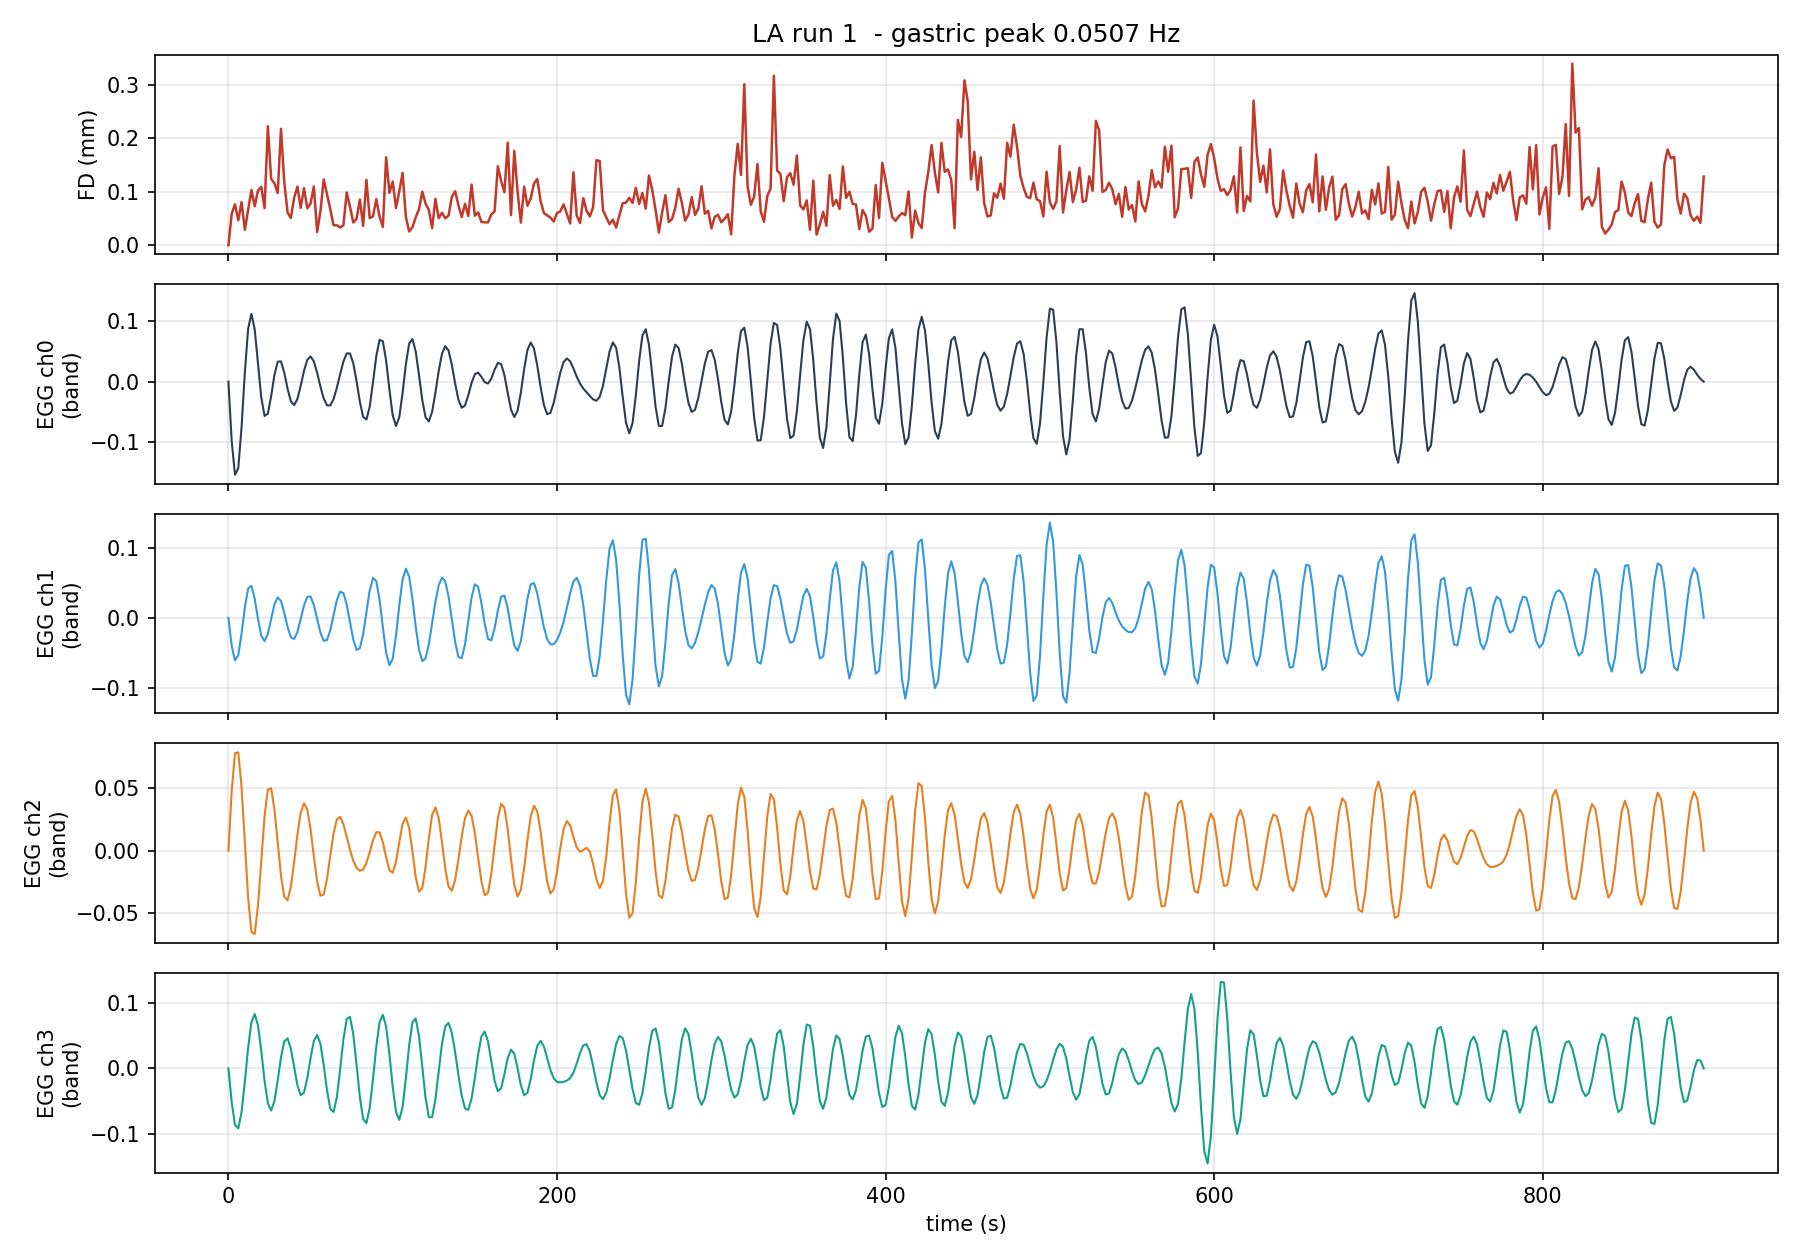
\includegraphics[width=0.95\linewidth]{outputs/fwd_overlay_LA_run1.png}
\caption{\textbf{Illustrative example from a single run} (\texttt{LA} run 1,
$n = 1$): FD (red, top) and the four bandpassed EGG channels (below).
Group-level summaries across all 84 runs are in
figures~\ref{fig:per_channel} and~\ref{fig:dom_vs_others}.}
\label{fig:overlay}
\end{figure}

Two further example overlays are in
\path{outputs/fwd_overlay_LA_run2.png} and
\path{outputs/fwd_overlay_BS_run1.png}.

\subsection{Channel-by-channel coupling}

Median coupling between FD and each individual EGG channel, across all
available runs:

\begin{table}[h!]
\centering
\small
\begin{tabular}{r r S[table-format=1.3] S[table-format=1.3] S[table-format=+1.3]}
\toprule
Channel & n & {PLV (median)} & {Coherence (median)} & {Pearson $r$ (median)} \\
\midrule
0 & 84  & 0.025 & 0.083 & -0.008 \\
1 & 84  & 0.024 & 0.093 & -0.001 \\
2 & 84  & 0.029 & 0.084 &  0.007 \\
3 & 75  & 0.022 & 0.079 & -0.008 \\
\bottomrule
\end{tabular}
\end{table}

The four channels look broadly interchangeable: PLV medians lie in a
narrow band (0.022--0.029), coherence medians in 0.079--0.093, and
Pearson $r$ medians sit near zero. The full distributions are below.

\begin{figure}[h!]
\centering
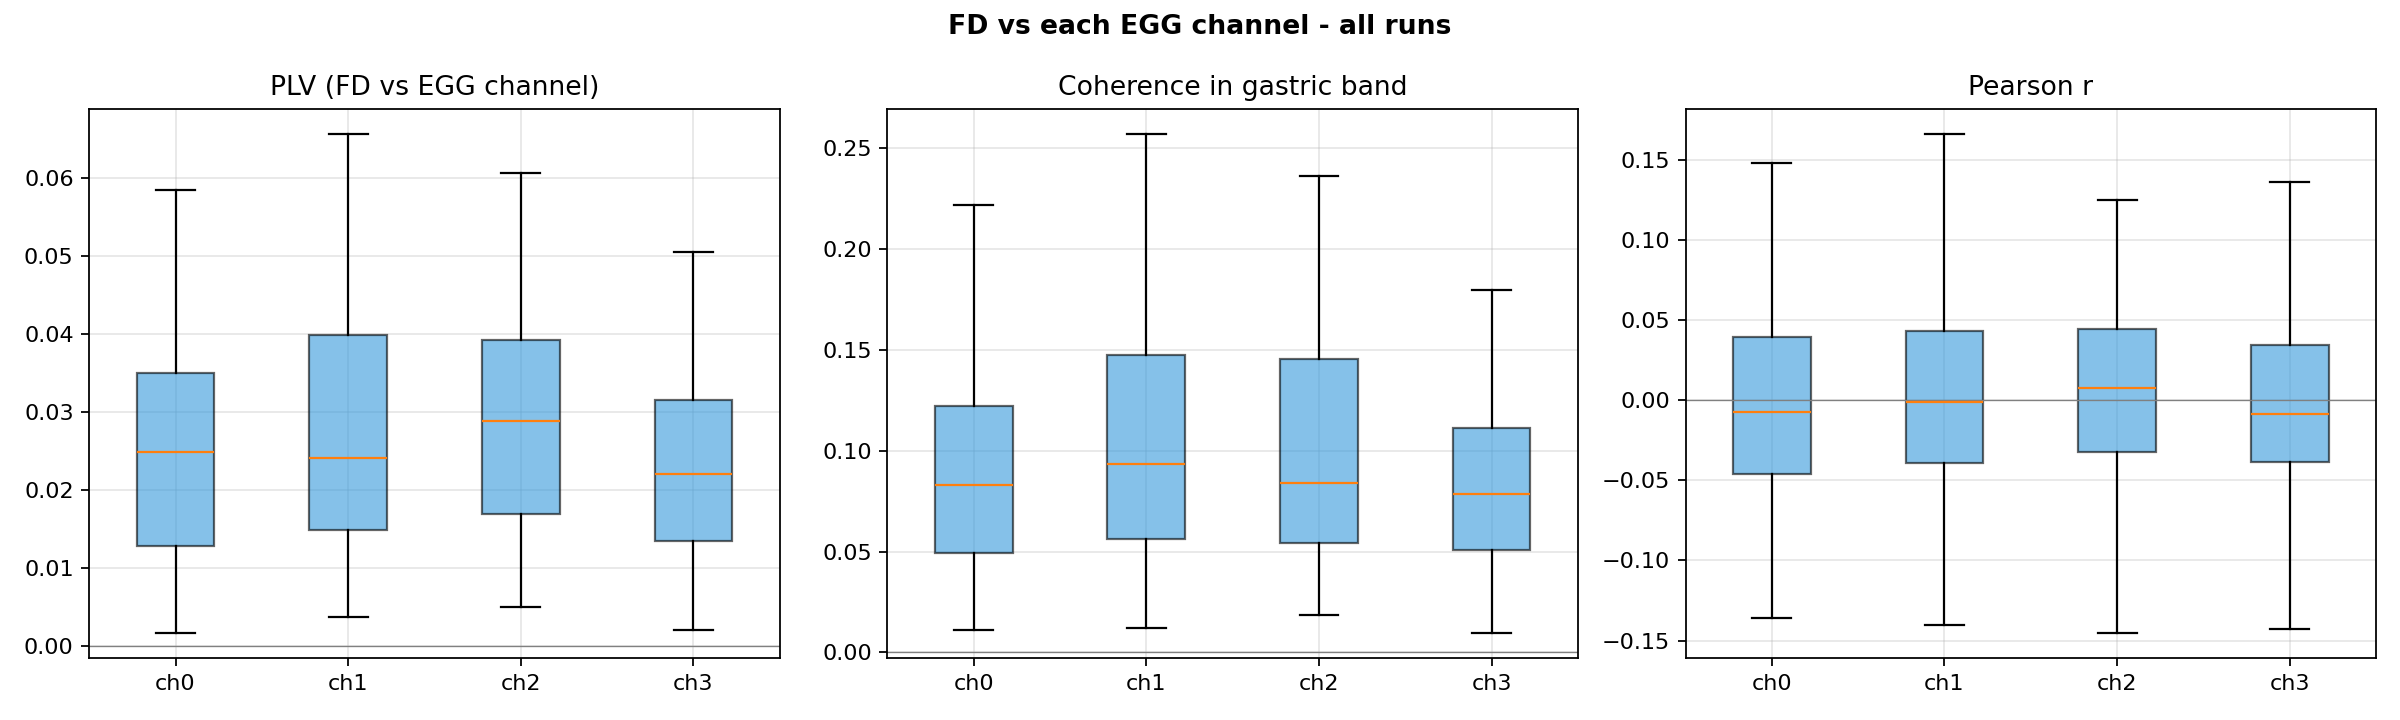
\includegraphics[width=0.95\linewidth]{outputs/fwd_channel_comparison.png}
\caption{FD vs each EGG channel: per-channel boxplots of PLV (left),
coherence in the gastric band (middle), and Pearson $r$ (right).
\textbf{$n = 84$ runs} per box (channels 0--2) and \textbf{$n = 75$ runs}
for channel 3 (some runs only have 3 active EGG electrodes).}
\label{fig:per_channel}
\end{figure}

\clearpage

\subsection{Does the dominant-channel choice matter?}

If the OHBM pipeline's dominant-channel pick captured a special FD
signal, the ``dominant'' boxes in the figure below would sit visibly
above the ``other electrodes'' boxes. They do not.

\begin{table}[h!]
\centering
\small
\begin{tabular}{l r S[table-format=1.3] S[table-format=1.3] S[table-format=+1.3]}
\toprule
& n & {PLV (median)} & {Coherence (median)} & {Pearson $r$ (median)} \\
\midrule
dominant electrode & 84  & 0.026 & 0.080 & -0.005 \\
other electrodes   & 243 & 0.025 & 0.087 & -0.001 \\
\bottomrule
\end{tabular}
\end{table}

\begin{figure}[h!]
\centering
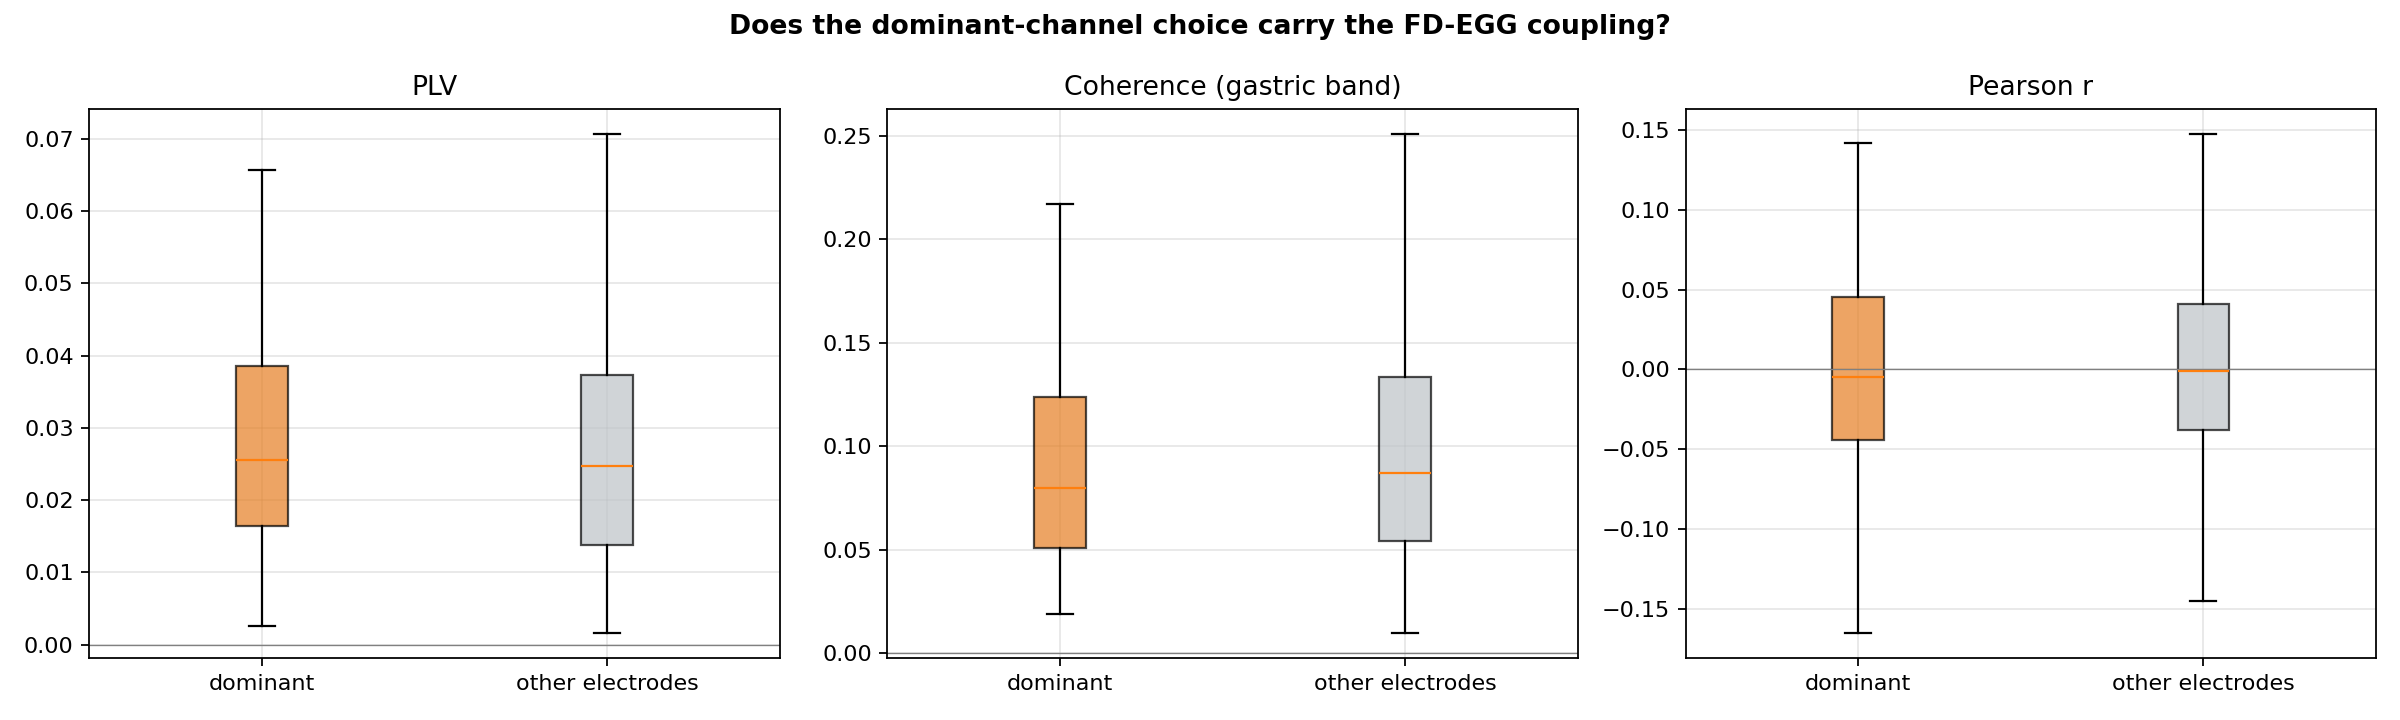
\includegraphics[width=0.95\linewidth]{outputs/fwd_dominant_vs_all.png}
\caption{Dominant electrode (orange) vs the other electrodes (grey)
for PLV (left), coherence in band (middle), and Pearson $r$ (right).
\textbf{$n = 84$ dominant rows, $n = 243$ other-electrode rows} across
all 84 runs.}
\label{fig:dom_vs_others}
\end{figure}

A separate way to ask the same question: in how many runs does the
data-detected dominant channel coincide with the channel that has the
strongest FD coupling?

\begin{itemize}
\item dominant $=$ argmax over channels of FD-EGG PLV: 23 / 84 runs
(27.4\%).
\item dominant $=$ argmax over channels of FD-EGG coherence: 22 / 84
runs (26.2\%).
\end{itemize}

With 4 channels the chance rate is 25\%, so the dominant pick does not
appear to track the FD-coupled channel. That may suggest the channel
that carries the most EGG power and the channel that couples best
with FD are roughly independent questions; either way, the choice of
dominant channel does not appear to bias the FD-EGG coupling result up
or down in a systematic way.

\section{Summary}

The mean and max FD on this dataset fall well within the range
Power et al.\ (2012) and Satterthwaite et al.\ (2013) report for
healthy adults at TR = 2~s. This observation may suggest that the FD
implementation behaves as expected for typical resting-state data.

The four cutaneous EGG channels appear to record the same $\sim$0.05~Hz
gastric slow wave: the bandpassed time courses overlay closely
(figure~\ref{fig:overlay}) and the coupling-with-FD distributions look
broadly interchangeable across channels.

The data-driven dominant channel (the one with the highest in-band EGG
variance) does not, on this dataset, coincide with the channel that
shows the strongest FD coupling more often than chance (about 26 to
27\% for 4 channels, compared with the 25\% chance rate). The
``dominant'' and ``other electrodes'' boxplots look similar across all
three coupling metrics. Together, these observations may suggest that
the OHBM pipeline's dominant-channel pick does not bias the FD vs EGG
coupling result up or down in any systematic way for these runs, and
that the four electrodes can be treated as roughly interchangeable for
this specific question.


\section*{References}

\begin{itemize}
\item Power JD \textit{et al.} (2012). Spurious but systematic
correlations in functional connectivity MRI networks arise from
subject motion. \textit{NeuroImage} 59(3):2142--2154.
\item Satterthwaite TD \textit{et al.} (2013). An improved framework
for confound regression and filtering for control of motion artifact in
the preprocessing of resting-state functional connectivity data.
\textit{NeuroImage} 64:240--256.
\item Choe AS \textit{et al.} (2021). Phase-locking of resting-state
brain networks with the gastric basal electrical rhythm. \textit{PLoS
ONE} 16(1):e0244756.
\item Levakov G, Ganor S, Avidan G (2023). Reliability and validity of
brain--gastric phase synchronization. \textit{Human Brain Mapping}
44:4956--4966.
\end{itemize}

\end{document}
